\PassOptionsToPackage{unicode=true}{hyperref} % options for packages loaded elsewhere
\PassOptionsToPackage{hyphens}{url}
%
\documentclass[ignorenonframetext,aspectratio=169]{beamer}
\usepackage{pgfpages}
\setbeamertemplate{caption}[numbered]
\setbeamertemplate{caption label separator}{: }
\setbeamercolor{caption name}{fg=normal text.fg}
\beamertemplatenavigationsymbolsempty
% Prevent slide breaks in the middle of a paragraph:
\widowpenalties 1 10000
\raggedbottom
\setbeamertemplate{part page}{
\centering
\begin{beamercolorbox}[sep=16pt,center]{part title}
  \usebeamerfont{part title}\insertpart\par
\end{beamercolorbox}
}
\setbeamertemplate{section page}{
\centering
\begin{beamercolorbox}[sep=12pt,center]{part title}
  \usebeamerfont{section title}\insertsection\par
\end{beamercolorbox}
}
\setbeamertemplate{subsection page}{
\centering
\begin{beamercolorbox}[sep=8pt,center]{part title}
  \usebeamerfont{subsection title}\insertsubsection\par
\end{beamercolorbox}
}
\AtBeginPart{
  \frame{\partpage}
}
\AtBeginSection{
  \ifbibliography
  \else
    \frame{\sectionpage}
  \fi
}
\AtBeginSubsection{
  \frame{\subsectionpage}
}
\usepackage{lmodern}
\usepackage{amssymb,amsmath}
\usepackage{ifxetex,ifluatex}
\usepackage{fixltx2e} % provides \textsubscript
\ifnum 0\ifxetex 1\fi\ifluatex 1\fi=0 % if pdftex
  \usepackage[T1]{fontenc}
  \usepackage[utf8]{inputenc}
  \usepackage{textcomp} % provides euro and other symbols
\else % if luatex or xelatex
  \usepackage{unicode-math}
  \defaultfontfeatures{Ligatures=TeX,Scale=MatchLowercase}
\fi
\usetheme[]{Frankfurt}
\usecolortheme{beaver}
% use upquote if available, for straight quotes in verbatim environments
\IfFileExists{upquote.sty}{\usepackage{upquote}}{}
% use microtype if available
\IfFileExists{microtype.sty}{%
\usepackage[]{microtype}
\UseMicrotypeSet[protrusion]{basicmath} % disable protrusion for tt fonts
}{}
\IfFileExists{parskip.sty}{%
\usepackage{parskip}
}{% else
\setlength{\parindent}{0pt}
\setlength{\parskip}{6pt plus 2pt minus 1pt}
}
\usepackage{hyperref}
\hypersetup{
            pdftitle={Bioethics in biotechnology},
            pdfauthor={Deependra Dhakal},
            pdfborder={0 0 0},
            breaklinks=true}
\urlstyle{same}  % don't use monospace font for urls
\newif\ifbibliography
\setlength{\emergencystretch}{3em}  % prevent overfull lines
\providecommand{\tightlist}{%
  \setlength{\itemsep}{0pt}\setlength{\parskip}{0pt}}
\setcounter{secnumdepth}{0}

% set default figure placement to htbp
\makeatletter
\def\fps@figure{htbp}
\makeatother

\usepackage{booktabs}
\usepackage{longtable}
\usepackage{array}
\usepackage{multirow}
\usepackage{wrapfig}
\usepackage{float}
\usepackage{colortbl}
\usepackage{pdflscape}
\usepackage{tabu}
\usepackage{threeparttable}
\usepackage{threeparttablex}
\usepackage[normalem]{ulem}
\usepackage{makecell}
\usepackage{xcolor}

% % set background image if you will
% \usebackgroundtemplate%
% {%
%     \includegraphics[width=\paperwidth,height=\paperheight]{02-dna_modification_background_dna_helix.jpg}%
% }

% % set background in a TikZ node for modifications
% % set background in a TikZ node for modifications
\usepackage{tikz}
\usepackage[absolute,overlay]{textpos}
\setbeamertemplate{title page}{
\tikz\node[opacity=0.9] {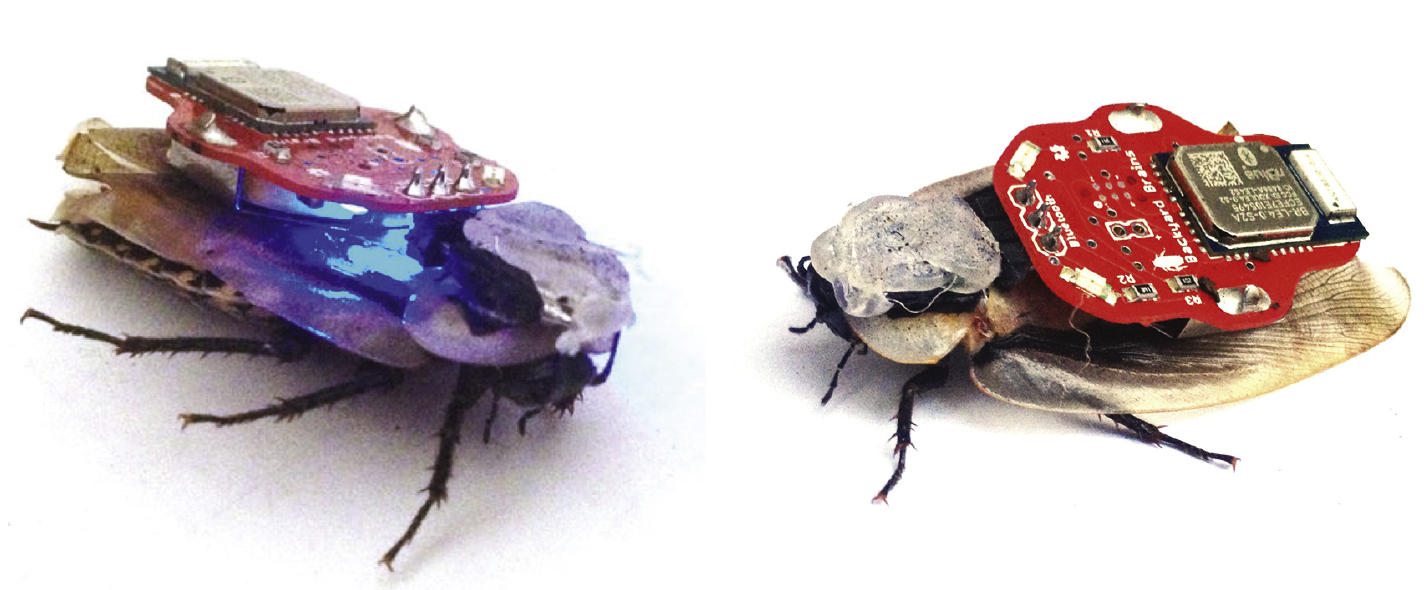
\includegraphics[width=0.8\paperwidth]{./07-bioethics_cover.png}};
% \tikz\node[opacity=0.8] {\includegraphics[width=5cm,ext=.1-overview_mutation_cover.png,type=png,read=.1-overview_mutation_cover.png]{1}} % if name shall contain dots, suppose filename = 01.1-overview_mutation_cover.png
\begin{textblock}{20}(1.5,2.8)\usebeamerfont{title} % 1.5 is x position in page
{\color{blue}\raggedright\par\inserttitle}
\end{textblock}
\begin{textblock}{7.5}(1.5,7) % 1.5 is x position in page
{\color{gray}\raggedright{\insertauthor}\mbox{}\\[0.2cm]
\insertdate}
\end{textblock}} % dd_rookie modified, figure is top aligned

% % set caption font size
% % note that beamer presentation native captions have their own configs
% \usepackage{caption}
% \captionsetup{font=footnotesize}

% this font option is amenable for beamer
\setbeamerfont{caption}{size=\tiny}

% some beamer themes naturally might not support navigation symbols
% \setbeamertemplate{navigation symbols}{} % remove navigation symbols

\setbeamertemplate{footline}[page number] % insert page number in footline

% \setbeamertemplate{navigation symbols}{slide} % insert slide indication in navigation
% \setbeamertemplate{navigation symbols}{frame} % insert frame indication in navigation
% \setbeamertemplate{navigation symbols}{section} % insert section indication in navigation
% \setbeamertemplate{navigation symbols}{subsection} % insert subsection indication in navigation

% \AtBeginSubsection{} % supress subsection display

\title{Bioethics in biotechnology}
\author{Deependra Dhakal}
\providecommand{\institute}[1]{}
\institute{GAASC, Baitadi \and Tribhuwan University}
\date{Academic year 2019-2020}

\begin{document}
\frame{\titlepage}

\begin{frame}
\tableofcontents[hideallsubsections]
\end{frame}
\hypertarget{introduction}{%
\section{Introduction}\label{introduction}}

\hypertarget{principles}{%
\subsection{Principles}\label{principles}}

\begin{frame}{Background}
\protect\hypertarget{background}{}

\framesubtitle{Why be ethical?}

\begin{itemize}
\tightlist
\item
  As biotechnology continues its march forward, it will inevitably raise
  new moral and legal questions.
\item
  There are few ``black and white'' issues in bioethics, but instead
  varying shades of gray.
\item
  Questions such as:

  \begin{itemize}
  \tightlist
  \item
    Who should control technology ?
  \item
    Who should be excluded or permitted, and who should decide ?
  \item
    Who should profit ?
  \item
    Should access to novel technology be made affordable ?
  \item
    Who should pay for the technology ?
  \end{itemize}
\item
  Much of ``official'' regarded bioethics derives from clinical
  biotechnology.
\end{itemize}

\end{frame}

\begin{frame}{Principles of bioethics}
\protect\hypertarget{principles-of-bioethics}{}

\begin{block}{Ethics}
"The philosophical study of the moral value of human conduct and of the rules and principles that ought to govern it; moral philosophy"
\end{block}

\begin{itemize}
\tightlist
\item
  The National Commission for the Protection of Human Subjects of
  Biomedical and Behavioral Research issued the Belmont Report in 1979.
  Although primarily aimed at biomedical research with human subjects,
\item
  Its basic principles-- \emph{autonomy}, \emph{beneficence}, and
  \emph{justice} Belmont Report in 1979 -- have often been applied to
  the broader areas of biotechnology.
\item
  Autonomy refers to informed consent and related issues and applies
  especially to medical research and clinical applications.
\item
  Privacy and confidentiality receive greater emphasis in biotechnology.
  In particular, access to personal genome information has become a
  thorny problem.
\item
  Beneficence involves promoting benefit and avoiding harm to people
  (and animals)---physically, mentally, and to their rights.
\end{itemize}

\end{frame}

\begin{frame}{Precautionary principle}
\protect\hypertarget{precautionary-principle}{}

\begin{itemize}
\tightlist
\item
  The precautionary principle states that if a proposed change has a
  possible risk of causing harm to people or to the environment, the
  burden of proving that it is safe (or very unlikely to cause harm)
  falls on those proposing the change.
\item
  In biotechnology the precautionary principle has been applied to such
  issues as

  \begin{itemize}
  \tightlist
  \item
    Spreading disease accidentally by using technology (such as the
    transmission of AIDS or hepatitis by blood transfusions or the
    emergence of mad cow disease by changing animal food processing).
  \item
    Introducing new pharmaceutical products, especially those generated
    by genetic engineering. Requiring pharmaceutical companies to
    perform clinical trials to show that new medications are safe is a
    well-established practice.
  \item
    Introducing genetically modified organisms into the environment.
  \item
    Creating artificial life.
  \end{itemize}
\end{itemize}

\end{frame}

\begin{frame}{Declaration}
\protect\hypertarget{declaration}{}

\begin{itemize}
\tightlist
\item
  In 2005, the United Nations issued a \textbf{Universal Declaration on
  Bioethics and Human Rights}, including a much-expanded set of
  principles:
\end{itemize}

\begin{columns}[T,onlytextwidth]
  
  \column{0.2\textwidth}
  \alert {General Provisions}
  \tiny{
  \begin{itemize}
  \item Article 1 Scope
  \item Article 2 Aims
  \end{itemize}
  }
  
  \column{0.4\textwidth}
  \alert {Principles}
  \tiny{
  \begin{itemize}
  \item Article 3 Human dignity and human rights
  \item Article 4 Benefit and harm
  \item Article 5 Autonomy and individual responsibility
  \item Article 6 Consent
  \item Article 7 Persons without capacity to consent
  \item Article 8 Respect for human vulnerability and personal integrity
  \item Article 9 Privacy and confidentiality
  \end{itemize}
  }
  
  \column{0.4\textwidth}
  
  \tiny{
  \begin{itemize}
  \item Article 10 Equality, justice and equity
  \item Article 11 Non-discrimination and non-stigmatization
  \item Article 12 Respect for cultural diversity and pluralism
  \item Article 13 Solidarity and cooperation
  \item Article 14 Social responsibility and health
  \item Article 15 Sharing of benefits
  \item Protecting future generations
  \item Protection of the environment, the biosphere and biodiversity
  \end{itemize}
  }

\end{columns}

\end{frame}

\hypertarget{power-of-information}{%
\section{Power of information}\label{power-of-information}}

\hypertarget{use-and-misuse-of-digital-information}{%
\subsection{Use and misuse of digital
information}\label{use-and-misuse-of-digital-information}}

\begin{frame}{Privacy and personal genetic information}
\protect\hypertarget{privacy-and-personal-genetic-information}{}

\begin{itemize}
\tightlist
\item
  What are the ethical implications of possessing, or being denied
  access to certain types of biological information.
\item
  Settlement of criminal cases
\item
  Creation of national criminal DNA database\ldots{}is it ethical?
\item
  Identity theft and digital infromation hack
\item
  In future it may be possible to predict potential health problems by
  analyzing individual's DNA (now being done for Huntington's disease).
  However, many people prefer not to know!
\item
  Personal genetic information is used by health care providers,
  insurance companies, government database.
\item
  Does government possessing genetic information constitute invasion of
  privacy ?
\item
  Legislation regarding use of genetic information has been passed in
  US: Genetic Information Nondiscrimination Act, 2008.
\end{itemize}

\end{frame}

\begin{frame}{The problem of dual-use research}
\protect\hypertarget{the-problem-of-dual-use-research}{}

\begin{itemize}
\tightlist
\item
  The World Health Organization defines
\end{itemize}

\begin{block}{Dual use research of concern (DURC)} 
Life sciences research that is intended for benefit, but which might easily be misapplied to do harm.
\end{block}

\begin{itemize}
\tightlist
\item
  Factors of consideration for DURC:

  \begin{itemize}
  \footnotesize{
  \item Increasing the harmful consequences of a biological agent or toxin.
    \item Disrupting immunity (or effective immunization) toward a biological agent or toxin.
    \item Making a biological agent or toxin resistant to useful preventative or therapeutic countermeasures.
    \item Improving the ability of a biological agent or toxin to evade detection.
    \item Improving the stability or transmissibility of a biological agent or toxin.
    \item Altering the host range (including tropism to particular tissues within the body) of a biological agent or toxin.
    \item Enhancing the susceptibility of a target population to a biological agent or toxin.
    \item Generating a novel pathogenic agent or toxin.
    \item Re-creating an extinct or eradicated pathogenic agent or toxin.
  }
    \end{itemize}
\end{itemize}

\end{frame}

\begin{frame}{Ownership of genetic information}
\protect\hypertarget{ownership-of-genetic-information}{}

\begin{itemize}
\tightlist
\item
  In the United States, products of nature cannot be patented, but until
  very recently, human gene sequences could.
\item
  The company Myriad Genetics patented the DNA sequences of two genes
  linked to breast cancer, BRCA1 and BRCA2. The company also developed a
  diagnostic assay based on these gene sequences. Thus, the effect of
  the patents was to eliminate all competition from the market because
  no other company could create a DNA-based test for these breast cancer
  genes.
\item
  Should scientists working at universities with public funding be
  allowed to patent their discoveries ?
\end{itemize}

\end{frame}

\hypertarget{possible-dangers-to-health-from-biotechnology}{%
\section{Possible dangers to health from
biotechnology}\label{possible-dangers-to-health-from-biotechnology}}

\hypertarget{creating-a-healthy-future}{%
\subsection{Creating a healthy future}\label{creating-a-healthy-future}}

\begin{frame}{Biological weapons}
\protect\hypertarget{biological-weapons}{}

\begin{figure}
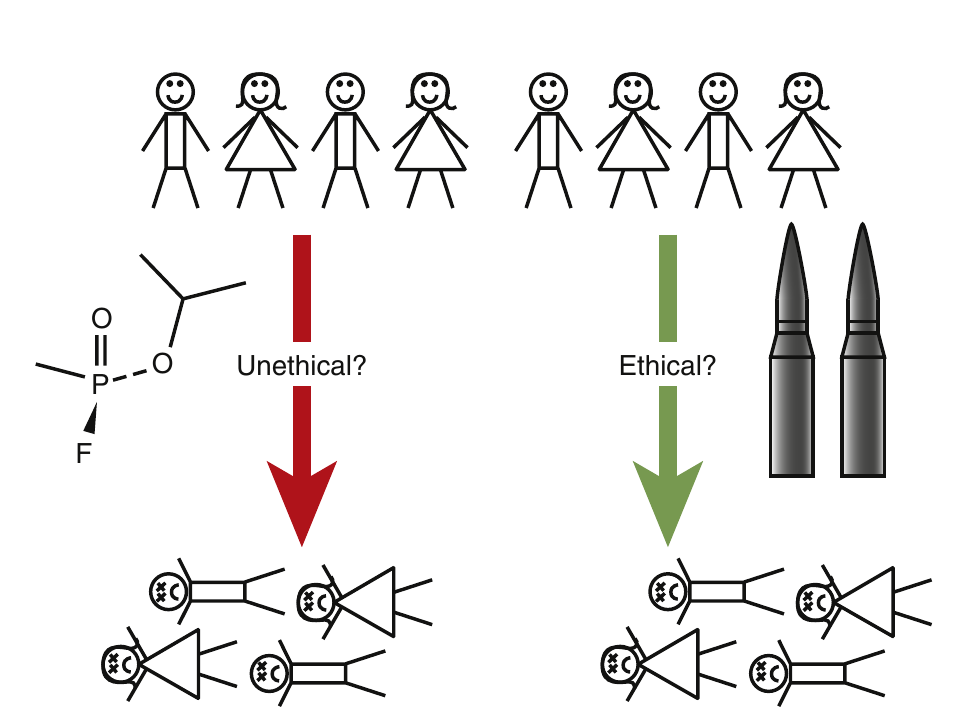
\includegraphics[width=0.28\linewidth]{../images/biological_weapon} \caption{\textbf{Syrian civil war} The victims are just as dead whether killed 'ethically' by bullets or 'unethically' by sarin nerve gas.}\label{fig:biofuel-production}
\end{figure}

\begin{itemize}
\tightlist
\item
  Anthrax attack in US in 2001. Are biological weapons more
  ``destructive'' or more ``scarier''?
\end{itemize}

\end{frame}

\begin{frame}{Antibiotic and antiviral resistance}
\protect\hypertarget{antibiotic-and-antiviral-resistance}{}

\begin{itemize}
\tightlist
\item
  MSRA; Tuberculosis
\item
  The United States in 2009 consumed over 36 million pounds of
  antibiotics, only 20\% of which were administered to humans.
\item
  Overprescription and underprescription
\item
  Retroviral therapies
\end{itemize}

\end{frame}

\hypertarget{genetically-modified-organisms}{%
\section{Genetically modified
organisms}\label{genetically-modified-organisms}}

\hypertarget{playing-with-nature}{%
\subsection{Playing with nature}\label{playing-with-nature}}

\begin{frame}{Transgenic plants}
\protect\hypertarget{transgenic-plants}{}

\begin{itemize}
\tightlist
\item
  Haven't humans been already practicing artificial monocultures,
  historically?
\item
  Are the adamant opposition of environmental and consumer groups
  against GMOs scientifically grounded?
\item
  According to the International Service for the Acquisition of
  Agribiotech Applications (ISAAA), 20 developing nations grow 52\% of
  the world's GMOs, while 8 developed nations grow the remaining 48\%.
\item
  The case of \emph{terminator seed}
\item
  US has 93\% of Soybeans, 80\% of Cotton and 80\% of Corn acerage
  planted with GMO crops.
\end{itemize}

\end{frame}

\begin{frame}{Transgenic animals}
\protect\hypertarget{transgenic-animals}{}

\begin{columns}[T,onlytextwidth]
  
  \column{0.6\textwidth}
  \begin{itemize}
    \item If we do not grow as much corn as we do today, European corn borer insects will likely be a rare insect.
    \item it has been proposed that manipulating Hox genes could “de-evolve” a chicken to a more ancestral form that somewhat resembles a dinosaur
    \item GFP bunny project
    \item Is it ethical to genetically modify animals for purely aesthetic reasons?
  \end{itemize}
  
  \column{0.4\textwidth}

\begin{figure}
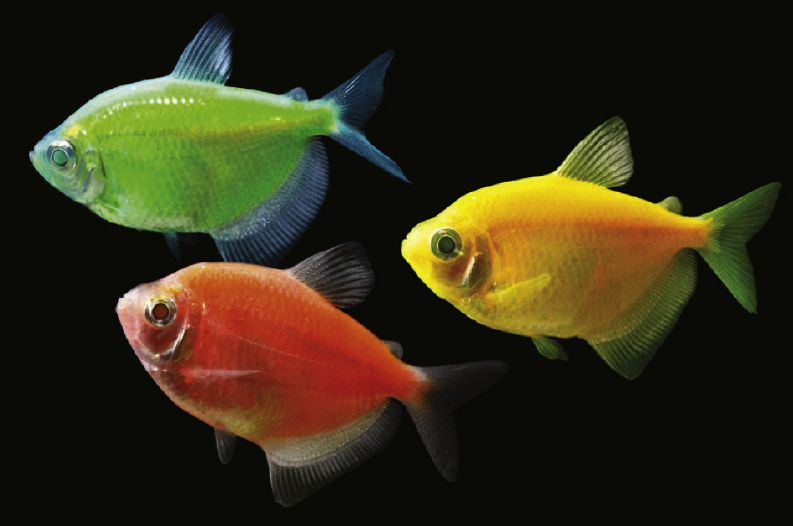
\includegraphics[width=0.5\linewidth]{../images/glofish_tetra} \caption{\textbf{GloFish Tetra} \newline You can purchase transgenic animals for your children's amusement and enlightenment! Courtesy of GloFish; http://www.glofish.com/meet-glofish/glofish-gallery/.}\label{fig:glofish-tetra}
\end{figure}

\end{columns}

\end{frame}

\begin{frame}{De-extinction}
\protect\hypertarget{de-extinction}{}

\begin{figure}
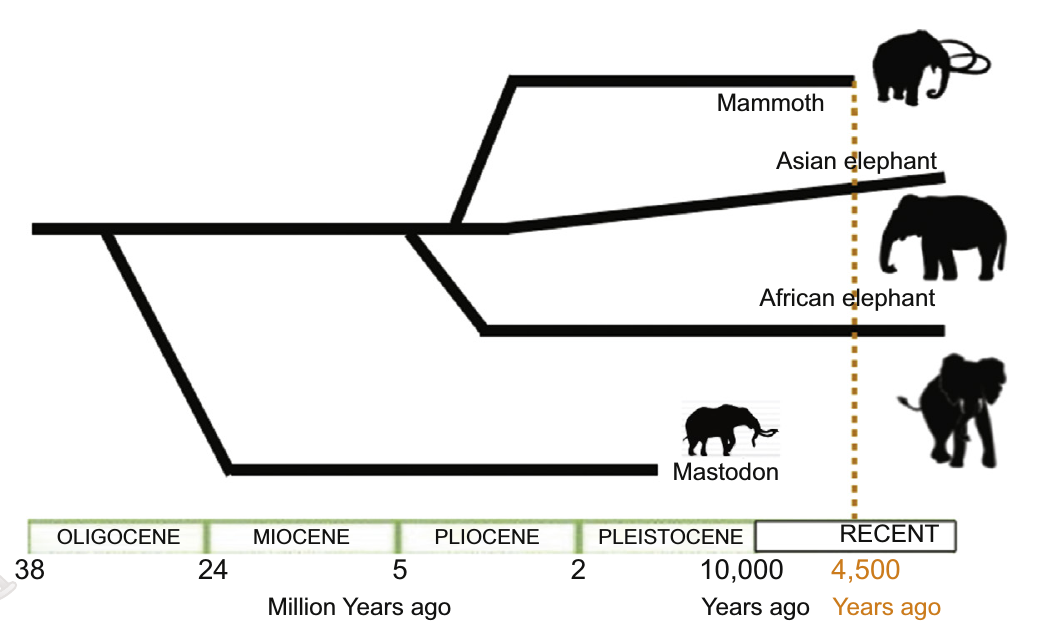
\includegraphics[width=0.45\linewidth]{../images/mammoth_deextinction} \caption{\textbf{Mammoth and elephant evolution} The extinct mammoth is actually more closely related to the Asian elephant than the Asian and African elephants are to each other. Note also that modern-day elephants are larger than the mammoth, which in turn was larger than the mastodon.}\label{fig:mammoth-resurrection}
\end{figure}

\end{frame}

\hypertarget{human-enhancement-cloning-and-engineering}{%
\section{Human enhancement, cloning and
engineering}\label{human-enhancement-cloning-and-engineering}}

\hypertarget{eugenics}{%
\subsection{Eugenics}\label{eugenics}}

\begin{frame}{Avenues}
\protect\hypertarget{avenues}{}

\begin{itemize}
\tightlist
\item
  Pregnancy screening
\item
  Stem cell therapy
\item
  Human genetic enhancement and cyborgs
\item
  Human cloning
\item
  Human genetic engineering
\end{itemize}

\end{frame}

\hypertarget{bibliography}{%
\section{Bibliography}\label{bibliography}}

\end{document}
